\begin{center}
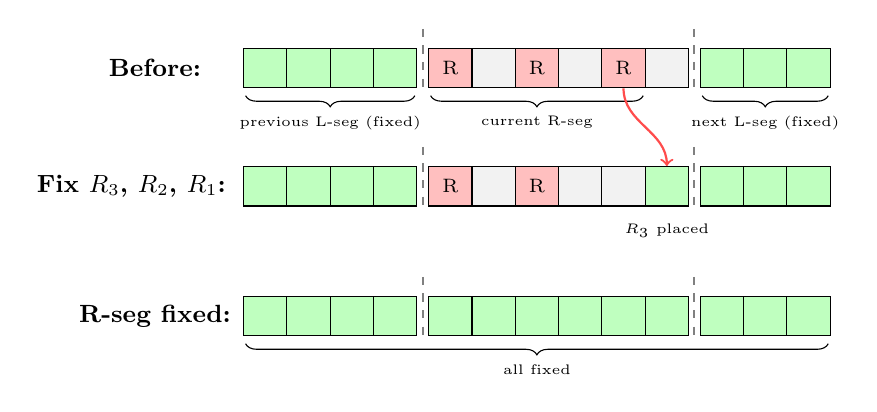
\begin{tikzpicture}[
    cell/.style={minimum width=0.55cm, minimum height=0.5cm, draw, font=\scriptsize},
    fixed/.style={cell, fill=green!25},
    current/.style={cell, fill=red!25},
    pending/.style={cell, fill=red!25},
    clean/.style={cell, fill=gray!10},
    arrow/.style={->, thick, red!70},
    boundary/.style={dashed, thick, black!50}
]
% Row 1: Before state
\node[font=\small\bfseries] at (-1.4, 0) {Before:};
\node[fixed] (f1) at (0, 0) {};
\node[fixed] (f2) at (0.55, 0) {};
\node[fixed] (f3) at (1.1, 0) {};
\node[fixed] (f4) at (1.65, 0) {};

% Boundary after green
\draw[boundary] (2.0, 0.5) -- (2.0, -0.3);

\node[pending] (r1) at (2.35, 0) {R};
\node[clean] (c1) at (2.9, 0) {};
\node[pending] (r2) at (3.45, 0) {R};
\node[clean] (c2) at (4.0, 0) {};
\node[current] (rcur) at (4.55, 0) {R};
\node[clean] (c3) at (5.1, 0) {};

% Boundary before next L-segment (already fixed)
\draw[boundary] (5.45, 0.5) -- (5.45, -0.3);

\node[fixed] (nl1) at (5.8, 0) {};
\node[fixed] (nl2) at (6.35, 0) {};
\node[fixed] (nl3) at (6.9, 0) {};

% Labels row 1
\draw[decorate, decoration={brace, amplitude=4pt, mirror}] 
    (-0.25, -0.35) -- (1.9, -0.35) node[midway, below=4pt, font=\tiny] {previous L-seg (fixed)};
\draw[decorate, decoration={brace, amplitude=4pt, mirror}] 
    (2.1, -0.35) -- (4.8, -0.35) node[midway, below=4pt, font=\tiny] {current R-seg};
\draw[decorate, decoration={brace, amplitude=4pt, mirror}] 
    (5.55, -0.35) -- (7.15, -0.35) node[midway, below=4pt, font=\tiny] {next L-seg (fixed)};

% Row 2: Fix rightmost R
\node[font=\small\bfseries] at (-1.7, -1.5) {Fix $R_3$, $R_2$, $R_1$:};
\node[fixed] (mf1) at (0, -1.5) {};
\node[fixed] (mf2) at (0.55, -1.5) {};
\node[fixed] (mf3) at (1.1, -1.5) {};
\node[fixed] (mf4) at (1.65, -1.5) {};

\draw[boundary] (2.0, -1.0) -- (2.0, -1.8);

\node[pending] (mr1) at (2.35, -1.5) {R};
\node[clean] (mc1) at (2.9, -1.5) {};
\node[pending] (mr2) at (3.45, -1.5) {R};
\node[clean] (mc2) at (4.0, -1.5) {};
\node[clean] (mc3) at (4.55, -1.5) {};
\node[fixed] (mrcur) at (5.1, -1.5) {};

\draw[boundary] (5.45, -1.0) -- (5.45, -1.8);

\node[fixed] (mnl1) at (5.8, -1.5) {};
\node[fixed] (mnl2) at (6.35, -1.5) {};
\node[fixed] (mnl3) at (6.9, -1.5) {};

% Arrow for movement
\draw[arrow] (rcur.south) to[out=-90, in=90] (mrcur.north);

% Labels row 2
\node[font=\tiny, anchor=north] at (5.1, -1.85) {$R_3$ placed};

% Row 3: After current segment fully fixed
\node[font=\small\bfseries, align=right] at (-1.4, -3.15) {R-seg fixed:};
\node[fixed] (af1) at (0, -3.15) {};
\node[fixed] (af2) at (0.55, -3.15) {};
\node[fixed] (af3) at (1.1, -3.15) {};
\node[fixed] (af4) at (1.65, -3.15) {};

\draw[boundary] (2.0, -2.65) -- (2.0, -3.45);

\node[fixed] (af5) at (2.35, -3.15) {};
\node[fixed] (af6) at (2.9, -3.15) {};
\node[fixed] (af7) at (3.45, -3.15) {};
\node[fixed] (af8) at (4.0, -3.15) {};
\node[fixed] (af9) at (4.55, -3.15) {};
\node[fixed] (af10) at (5.1, -3.15) {};

\draw[boundary] (5.45, -2.65) -- (5.45, -3.45);

\node[fixed] (af11) at (5.8, -3.15) {};
\node[fixed] (af12) at (6.35, -3.15) {};
\node[fixed] (af13) at (6.9, -3.15) {};

% Labels row 3
\draw[decorate, decoration={brace, amplitude=4pt, mirror}] 
    (-0.25, -3.5) -- (7.15, -3.5) node[midway, below=4pt, font=\tiny] {all fixed};
\end{tikzpicture}
\end{center}